\documentclass[12pt,a4paper]{standalone}
\usepackage[utf8]{inputenc}
\usepackage[T1]{fontenc}
\usepackage{tikz}
\begin{document}
	
	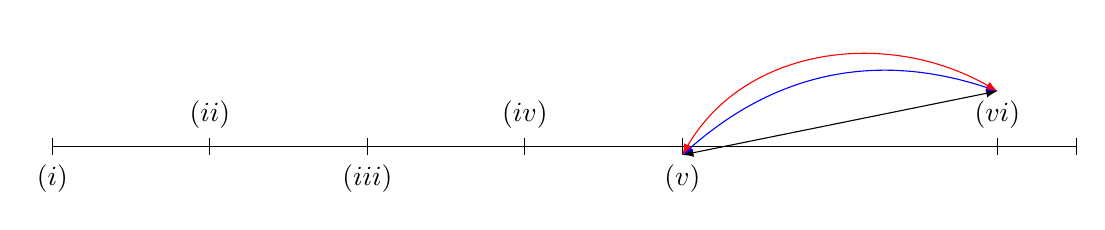
\begin{tikzpicture}
	\draw (0,0) -- (13,0);
	\foreach \x in {0,2,4,6,8,12,13}
	\draw (\x cm,3pt) -- (\x cm,-3pt);
	\draw (0,0) node[below=3pt] (a) {$(i)$} node[above=3pt] {};
	\draw (2,0) node[below=3pt] (b) {} node[above=3pt] {$(ii)$};
	\draw (4,0)  node[below=3pt]  {$(iii)$} node[above=3pt] (c) {};
	\draw (6,0) node[below=3pt](d) {} node[above=3pt] {$(iv)$};
	\draw (8,0) node[below=3pt](e) {$(v)$} node[above=3pt] {};
	\draw (12,0) node[above=3pt] (f) {$(vi)$} node[below=3pt] {};
	\draw[latex-latex]
	(e.north) -- (f.north);
	\draw[latex-latex,blue]
	(e.north) to[bend left] (f.north);
	\draw[latex-latex,red]
	(e.north) to[out=60,in=150] (f.north);
	\end{tikzpicture}\qquad
%	\begin{tikzpicture}
%	\draw (0,0) -- (13,0);
%	\foreach \x in {0,2,4,6,8,12,13}
%	\draw (\x cm,3pt) -- (\x cm,-3pt);
%	\draw (0,0) node[below=3pt] (a) {$(i)$} node[above=3pt] {};
%	\draw (2,0) node[below=3pt] (b) {} node[above=3pt] {$(ii)$};
%	\draw (4,0)  node[below=3pt]  {$(iii)$} node[above=3pt] (c) {};
%	\draw (6,0) node[below=3pt](d) {} node[above=3pt] {$(iv)$};
%	\draw (8,0) node[below=3pt](e) {$(v)$} node[above=3pt] {};
%	\draw (12,0) node[above=3pt] (f) {$(vi)$} node[below=3pt] {};
%	\draw[latex-latex]
%	(e.north|-f.north) -- (f.north);
%	\draw[latex-latex,blue]
%	(e.north|-f.north) to[bend left] (f.north);
%	\draw[latex-latex,red]
%	(e.north|-f.north) to[out=60,in=120] (f.north);
%	\end{tikzpicture}
	
\end{document}